
\chapter{PENDEKATAN\label{cha:3-Metodologi}}


\section{Motivasi \label{sec:3-Motivasi}}

Motivasi dari Metodologi


\section{Framework Riset\label{sub:3-Framework}}

Isi tentang framework dari riset

\section{Pendekatan\label{sec:3-Pendekatan} }

\begin{figure}[!t]
\begin{center}\begin{tabular}{cc}
\subfloat[Agreement by using Algorithm]
{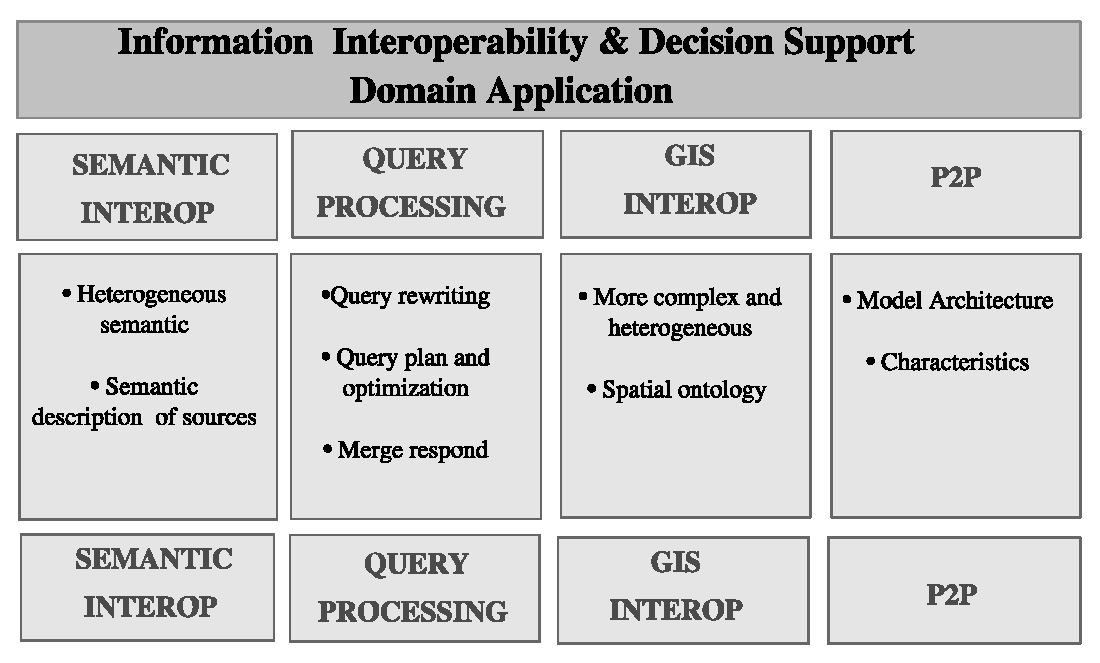
\includegraphics[width=0.4\columnwidth]{bab3/ContohGbr3_1.eps} \label{fig:3-noFCase1} }&
\subfloat[Agreement by using Algorithm and User feedback]
{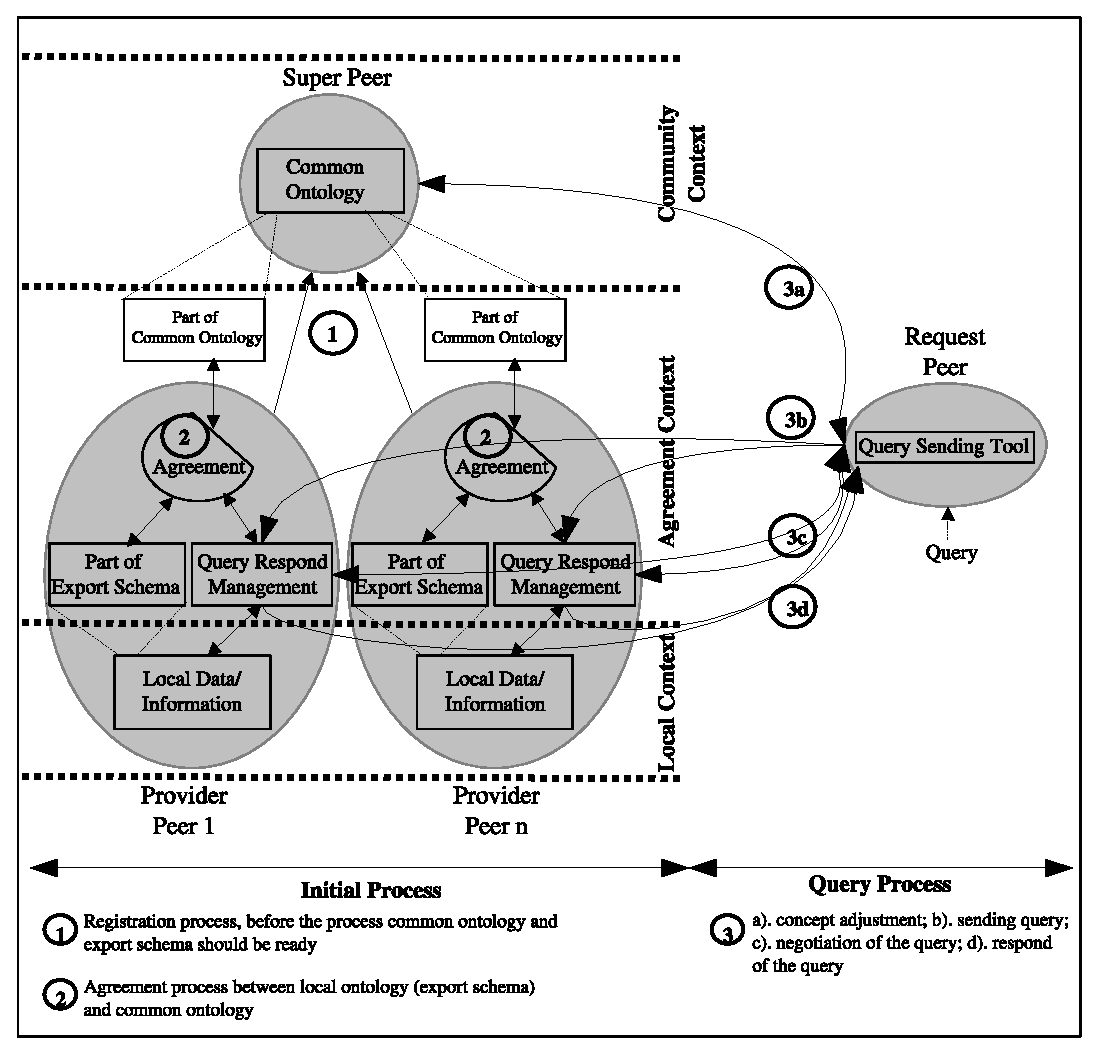
\includegraphics[width=0.4\columnwidth]{bab3/ContohGbr3_2.eps} \label{fig:3-FeedCase1} }\tabularnewline
&
\tabularnewline
\multicolumn{2}{c}
{
\subfloat[Manual mapping by Cruz et al]
{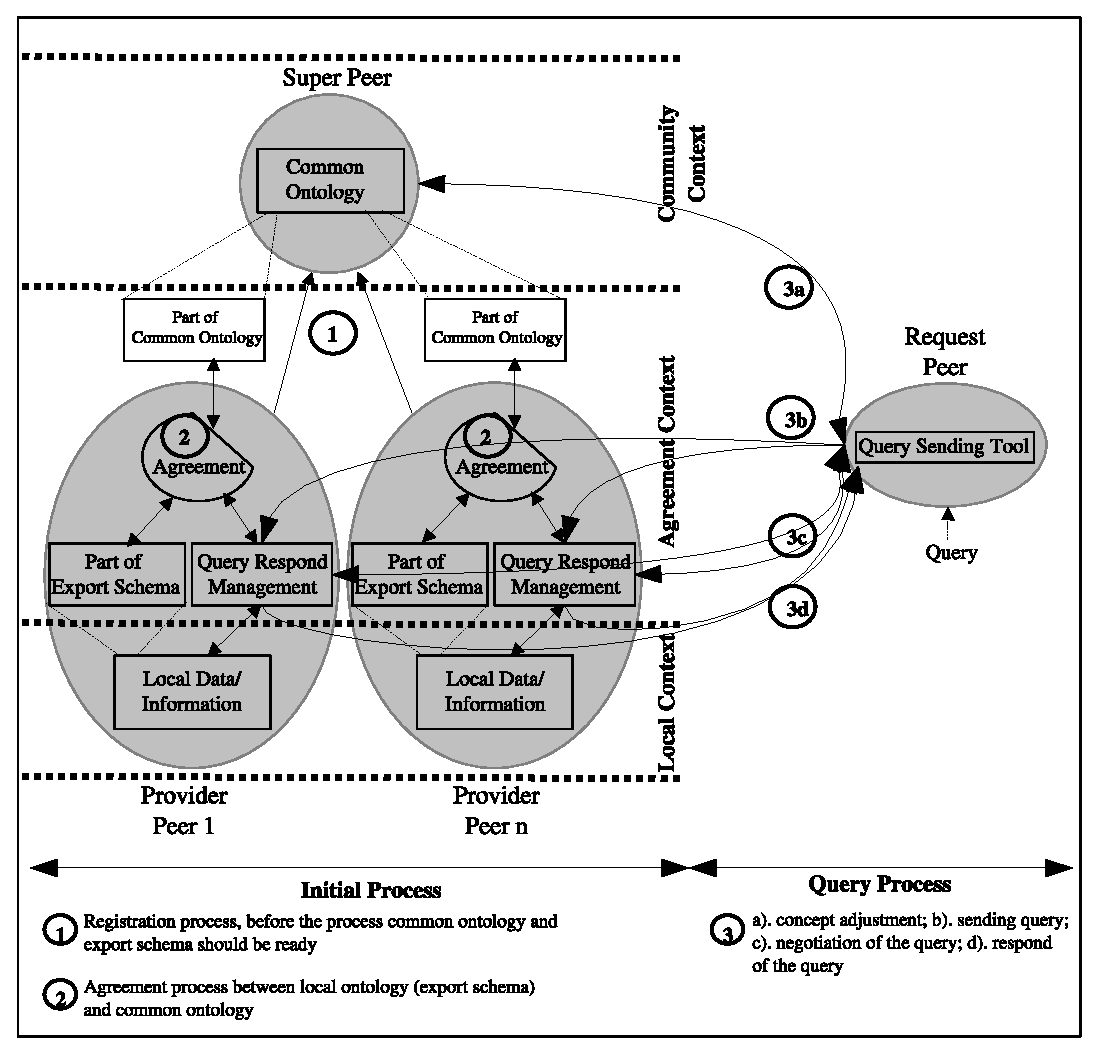
\includegraphics[width=0.4\columnwidth]{bab3/ContohGbr3_2.eps} \label{fig3-:CruzCase1} }
}\tabularnewline
\end{tabular}\end{center}
\vspace{-0.3cm}
\caption{Agreement Results on Case 1} \label{fig:3-Case1Result}
\vspace{-0.6cm}
\begin{center} \rule{0.0\columnwidth}{0.3pt} \end{center}
\end{figure}